%File: formatting-instruction.tex
\documentclass[letterpaper]{article}
\usepackage{aaai}
\usepackage{times}
\usepackage{helvet}
\usepackage{colortbl}
%\usepackage[style=apa,autocite=footnote]{biblatex}
\usepackage{comment}
\usepackage{appendix}
\usepackage{courier}
\usepackage{xcolor}
\usepackage{graphicx}
\graphicspath{ {./imgs/} }

\newcommand{\NIGMS}{\textsc{NIGMS}}
\newcommand{\openai}{\textsc{OpenAI}}
\newcommand{\guix}{\textsc{Guix}}
\newcommand{\project}{\textit{GeneNetwork.org Q\&A system}}
\newcommand{\hl}[1]{#1}
\newcommand{\GN}{{\textsc{GeneNetwork.org}}}
\newcommand{\lsRDF}{\LS{Wilkinson}}
\newcommand{\red}[1]{{\textcolor{red}{#1}}}
\newcommand{\cyan}[1]{{\textcolor{cyan}{#1}}}
\newcommand{\violet}[1]{{\textcolor{violet}{#1}}}
\newcommand{\brown}[1]{{\textcolor{brown}{#1}}}
\newcommand{\FIXME}[1]{\red{[FIXME: #1]}}

\frenchspacing
\setlength{\pdfpagewidth}{8.5in}
\setlength{\pdfpageheight}{11in}
\pdfinfo{
/Title (Insert Your Title Here)
/Author (Put All Your Authors Here, Separated by Commas)}
\setcounter{secnumdepth}{0}  
 \begin{document}
% The file aaai.sty is the style file for AAAI Press 
% proceedings, working notes, and technical reports.
%
\title{Generative AI In the pursuit to moderate and expose\\ Genetic/Genomic Knowledge}
\author{S. Solomon Darnell, Adrian Kibet(?), Brian PoppinTonic (?), Munyoki Kilyungi and Pjotr Prins\\
UTHSC Department of Genetics, Genomics and Informatics (GGI)\\
71 S. Manassas Street, 4th Floor\\
Memphis, Tennessee 38163\\
e $->$ genetics@uthsc.edu, ssd2023@nyeusi.tech
}
\maketitle
\begin{abstract}
\begin{quote}
The advent of popular and useful large text search and generative artificial intelligence (GAI) has led to the automation of many rote tasks and more amazingly multiple creative ones.
Generative artificial intelligence is based off of expansive machine learning models which exploded in relevance around fifteen years ago as convolutional neural nets (CNNs) began outperforming other methods in image classification tasks.
After a decade of wide-spanning, in research circles, development of deep learning networks (mostly underpinned by powerful convolutional neural networks) transformed into development of generative AI models.
ChatGPT, the leader of the pack in generative AI, is a private company that has curated extremely large models comprised of many billions of parameters.
The wild utility of generative AI models was made manifest to the world at large in late 2022, and what is following is a `mad dash' towards exploration, improvement, duplication and usage of generative AI systems. 
The department of genetics, genomics and informatics at the University of Tennessee Health Sciences center is no different as we are building an expert system that uses generative AI to bring knowledge and insights to people regardless of their level of ability or scientific knowledge.
\end{quote}
\end{abstract}

\section{Introduction}


\noindent Scholars world wide spend exhaustive amounts of time and effort reading, summarizing, converting, memorizing, and mixing knowledge for their own purposes, and to push science forward.
Since the inception of AI its promise has exponentially out-sized its capabilities; however, computing resources strong enough to exploit deep learning in conjunction with continual improvements in the use and management of `big data' have begun to close the gap between `perceived utility' and promise of AI.
`Perceived utility' is how the common person understands AIs use and helpfulness.
There are AI utilities, applications, and algorithms that are used widely for automation, recognition, navigation, semi-autonomous vehicles, mars rover exploration, deep question answering, and now creativity.
The essence of AI is getting computers to perform `intelligent' human tasks.
Pursuit of the same has caused some researchers to thoroughly examine and re-examine their definitions of intelligence.
Many see a humanoid android or automaton that is difficult to differentiate from a human as the pinnacle of AI; because AI as a field has so many areas in which it needs to improve to reach such a technical height, it is defined with many sub-fields.
The major sub-fields of AI include: machine learning, natural language processing, 
\cite{Azaria:2022} \cite{Zhang:2023} \cite{Foucart:2023} \cite{DePeau-Wilson:2023}

Since the deep learning boom in 2010, there has been a mad rush to apply and improve its techniques.
The first `killer' application was image classification, still and video.
Deep learning has made image classification so accurate until a large technology company has made it known that it has failed unless its `driverless' technology is the hallmark feature in its electric vehicles. 
Before the success of deep learning models on images classification attempts at `self-driving' vehicles failed or the idea was a `non-starter`.
As we tend to only hear about the most negative news, the existing Tesla `self-driving' cars are making moves on the road, mostly to the great delight of their owners.
Deep learning techniques have made the accuracy and error rate of many biometric technologies so enviable that many scientists consider some biometrics issues as solved, especially with modalities that are highly persistent, permanent and ubiquitous (e.g. iris, face, fingerprint).
As deep learning is being improved so goes the hardware used to run the necessary algorithms.

Consistently improving techniques and hardware leads to neural networks with billions of parameters instead of hundreds or thousands.
In the same vein, it seems that it takes a model with billions of parameters to really `understand' and respond using human language.

By training and painstakingly moderating humongous neural network modesl, OpenAI, was able to build what seems a quantum leap in the generative AI, ChatGPT a large language model that generates `mostly coherent' responses to human speech, without having anything close to a human curated script.
Although ChatGPT relies on a neural network model to accomplish its goals, it has popularized the term `large language model' (LLM).
In addition to creating a model that is magnificent at parsing information, understanding free-form human requests, and responding in a manner that can lead to the easy passing of the Turing test, OpenAI and others have trained neural network models on so many examples of data in different areas until `Generative AI' has pervaded the popular lexicon.
Generative AI (gAI) uses deep learning techniques to produce images, video, text, and more based on a free form query, making ChatGPT itself gAI.
Generative AI has recently gained attention due to the ability of services such as Midjourney (get ref) generating professional quality logos, portraits and other images based off of requests in free form human language.
The term `free form' is being used often as the generative models and LLMs do not need one to follow a script to generate output.

\begin{comment}
Thankfully AI is still an extremely hot topic; however, people are referring to everything that seems computationally smart as `artificial intelligence' (AI), mainly to keep things simple.
As stated in the introduction deep learning, mainly based on convolutional neural networks (CNNs), began showing breakthrough performance in image classification tasks, and scientists have been having a field day with the performance gains for multiple tasks, even in genomics [cite so many previous papers from the Diversity application write-up].
\end{comment}
\section{Current State-of-the-Art}

Artificial intelligence is a large research area that includes machine learning, and expert system topics~\cite{RussellNorvig:2016}.
Expert systems have two major components: an inference engine and a knowledge base~\cite{Liao:2005,Tan:2017}.
Machine learning models are best defined by their knowledge base, network architecture, activation function and number of parameters.
Machine learning techniques hae been applied to many areas of biological research \cite{Deng:2011,Angermueller:2016,Gawehn:2016_deep,Min:2017,Miotto:2018:deep,Tran:2018,Toh:2019,Zhang:2019,Bouwmeester:2020,Wen:2020:deep,Caudai:2021,Talukder:2021,Hassabis:2022} for the better part of the last decade.

\subsection{Large Language Models (\llms)}
Late 2022 saw an introduction to \llms\ that got the notice of the entire world \cite{Schulman:2022_chatgptintro}.
OpenAI debuted ChatGPT an `ask me anything' system that seemed to be the logical extension of good `search' and excellent `prompt' support, in the veins of an incredibly improved `Alexa' (by Amazon), `Siri' (by Apple) or `Cortana' (by Microsoft).
While these voice activated assistants seem `intelligent', they are programmed in a fashion that allows them to support very specific and directly encoded tasks, such as controlling `smart' devices (e.g. thermostats, lights, alarms, locks, speakers and televisions) \cite{Hoy:2018}.

Google Bard \cite{GoogleBard:2023}, Bing Chat \cite{BingChat:2023}, Dolly by Databricks \cite{Dolly:2023}, and Llama by Meta \cite{Llama:2023,Llama2:2023} are `big techs' answer to the previously rogue startup `OpenAI', as Microsoft has recently invested heavily \cite{Browne:2023}.
Many of the weights of the models are kept under wraps by their owners; however, Databricks and Meta have open-sourced their models, allowing people all over the world to experiment and extend a high quality LLM democratizing the technology.
OpenAI allows for a paid account to fine-tune their models for specific use-cases, but it has not open-sourced the model to enable others to run a full OpenAI \gpts\ model for themselves.
We will build and test using the open-source \llms.


\subsection{Causal Learning}
In their explanatory reference summary book for causal inference (CI), Pearl and Mackenzie~\cite{Pearl:2018} make the observation that machine learning algorithms and tools can `at best' provide a summary of data and/or transform it without using a model (of the precise problem domain).
In ML a `model' is an algorithm or set of algorithms trained to recognize a very limited sub-class of pattern.
It refers to a replica of the environmental and situational conditions that lead to an observable outcome or data at a manageable scale.
CI describes its usefulness using the `ladder of causation', which has three levels: association, intervention and counterfactuals \cite{Pearl:2018}.
An example of questions that can be answered by association:
\begin{itemize}
    \item What does a sore throat tell me about the severity of the flu?
    \item If I experience dizziness does that necessitate inner ear trouble?
\end{itemize}

Example questions that can be answered by intervention:
\begin{itemize}
    \item If I drink hot water with lemon and ginger will my cold symptoms disappear?
    \item Will taking the same Covid-19 vaccine 3 times ensure I'll never have "severe" Covid-19 symptoms?
\end{itemize}

Example questions that can be answered by deploying counterfactuals:
\begin{itemize}
    \item If I had done heavy exercise 6 times a week for the past decade, would I be an Olympic level athlete?
    \item If I had not been exposed to high levels of mosquito repellent and steel soot as a young child, would I still have asthma?
\end{itemize}

At the second level of the ladder of causation, intervention, the base data alone can not answer the question.
For instance, data can answer that many people reported feeling relief from cold symptoms, and tell us the percentage, possibly of people who gel better who have profiles similar to oneself.
Intervention questions are usually answered using experimentation, while with CI these questions will be answerable using its techniques.

As we found in the summary of deep learning in omics reviews people need to trust the data, algorithms and techniques used for translational medicine, phenotype prediction, precision medicine, advanced therapeutics and more.
A good way to understand is by asking ``why'', and as Judea Pearl \cite{Pearl:1995,Pearl:2009,Pearl:2019} has explained in his multiple works is by using causal inference.
It can argued that without a system being able to answer questions properly that include interventions and counterfactuals, the system can not truely have human level intelligence.
Computers have for a long time had better `memory' and `memory access speed' than humans, a fact proven by IBM's Watson in 2011~\cite{Ferrucci:2010_watson}; however, even given all of the data in the world, the current LLM based inferencing and optimized search and retrieval does not allow systems to answer counterfactuals and many non-popular intervention queries.
Therefore, in order to push \llms\ to an even more impressive path of meaning generation and inference is by including causal reasoning into the training or fine-tuning of huge foundation models.

\section{LLM Strengths}
\subsection{Generative AI for Creativity}

\begin{figure}[ht]
    
\includegraphics[width=8cm]{imgs/african_woman_steampunk.eps}
    \caption{African Woman in Steampunk Style}
\end{figure}

\begin{figure}[ht]
    
\includegraphics[width=8cm]{imgs/sudanese_solar_pyramid.eps}
    \caption{Sudanese Pyramid in a Modern style using Today's solar technology}
\end{figure}
\section{Weaknesses in LLMs}
Data is not referenced when answers are generated.
LLMs and generative AI have the same issues in that pure fact patterns are not mapped, similarities are mapped and based on the data available.
While the model is being trained

\section{Mitigating the weaknesses of an open LLM}
\subsection{How much data?}
ChatGPT was trained on multitudinous data scoured from all over the internet. 
With this almost indeterminate information grab comes petabytes of information, which required extreme effort to curate.
\subsection{Which data?}
Is all data good data?
Due to the nature of the world wide digital web (www) \textbf{bias} is prevalent, and training a model on highly biased information leads to biased results [mention the algorithmic justice league].
\subsection{Re-introducing Oracles}
In simple language a software Oracle is like an advanced lookup/hash table or data tuple where each entry has a single matter-of-fact answer.
An Oracle is generally a master of a special area of knowledge.
In the real world, an Oracle is an expert.
Medical practitioners are Oracles; however, they are Oracles with specializations concerning how different systems of the human body works and how it responds to multitudinous treatments.
There are many different types of medical practitioners, one group of which are nurses.
Nurses have different levels of expertise on the human body, how people react to treatment, real-life human-drug interactions, and sub-specialties, e.g. Renal nurse, Mid-wife (birthing) nurse, pediatric nurse, neonatal ICU nurse, emergency room nurse, oncology nurse, surgery nurse, post-surgery nurse, and so on.
Each nurse has different expertise that spans not only written medical knowledge, but also experience from interacting face-to-face with living patients.
People may have the same major malady yet need to be given differing treatments based on their personality traits, not any other underlying medical conditions.
Being able to encode this knowledge into an Oracle is nothing new, while it takes care and attention [cite many expert systems].
Part of the inference of an expert system is being able to, for example, take malady's and the knowledge of nurses to come up with the best treatment for an individual.
Also, it would be wonderful to be able to know how often a prescribed treatment works, and how well.

\begin{comment}
Each nurse has undergone specialized training to become and expert and then learned thru practice.
In nursing practice there are many variables involved when discerning and providing treatment.
A model is fed with knowledge, like a nurse being trained, and the models' practice is interacting with experts and being told whether or not the answers it is giving are correct given the query.
\end{comment}
\section{Innovations}

\subsection{Updating the Expert System}
In academia and industry the term expert system has lost its luster.
Expert systems ended up only seeming like experts to those with the vocabulary for the task for which it was designed.
AI researchers, before the age of ubiquitous deep learning, almost all have experience designing and building expert systems of one type or another, giving us insight on the strengths and weaknesses of these types of systems.
The main weaknesses of expert systems, before the age of \gpts, and latter, type \llms\  and powerful generative AI (\gai), are the inclusion of new information (data ingestion) and the ability to make smart inferences on all knowledge available to it.
\llms\ have an uncanny knack for information ingestion and inference; however, due to the way neural networks learn information perfect inference is not a possibility.
Because perfect inference is not possible even when deduced by models with billions of parameters, the expert system must guide the output of the model by querying a knowledge base of data on which the system is to be an expert.
\llms\ allow the interface to the expert system to be accessible by anyone who can speak a language that it can understand.
\llms\ understand natural language and can perform high-level inference in response to natural language making them an extremely important component of an evolved expert system.
An expert system requires an inference engine and a knowledge base.
Modern LLms provide the inference engine, while the knowledge based can be curated, and finally the process must be moderated such that LLM hallucination can not interfere with the results; because what use is an expert system that will not tell you the truth?

We follow a path similar to \cite{Karpas:2022:mrkl} at AI21, who have developed the Modular Reasoning, Knowledge and Language (MRKL) system, another LLM based chat and question answering system that uses `experts' to ensure the retrieval of factual information.
Software oracles are the different experts to whom you can ask questions in an expert system.
The system as it exists only relies on the documents on which it is trained to answer questions; however, being confined to just this is not close to being suitable for our use case.
Our use case being a system that is an overall expert concerning genetic and genomics research on rats and mice in the \GN\ database and ecosystem.
The experts in this research area have access to and knowledge of more than the documents that pertain to \GN\ but many scientific texts, publishing houses, knowledge bases and more.
For example, the Bing chat system uses wikipedia, a large online encyclopedia, and many online scientific sources.
The scientists that operate and maintain \GN\ have created metadata reference information, and other data points that can be added to the system and will create more of an oracle of the LLM trained system.
While other resources, line PubMed, have its own APIs so it is an open oracle that can be queried to support the \project.
%\subsection{Not Just Machine Learning (ML)}

A system should be built that supports researchers of varying levels of ability.
This system should be able to communicate well with people with differing levels of knowledge who seek variable levels of atomicity.
On the scale of accommodating people with differing levels of knowledge, Bing chat, co-developed by OpenAI and Microsoft, performs admirably.
When querying the system about a specific transcription factor, it not only provides a summarized description of the subject, but also returns citations as links.

%\newpage
%\captionsetup{font={scriptsize,sc,up,singlespacing}}
\begin{figure}[h] % Figure at bottom of the page ([b] argument, could be "t" for top or "h" for here)
	\centering
	%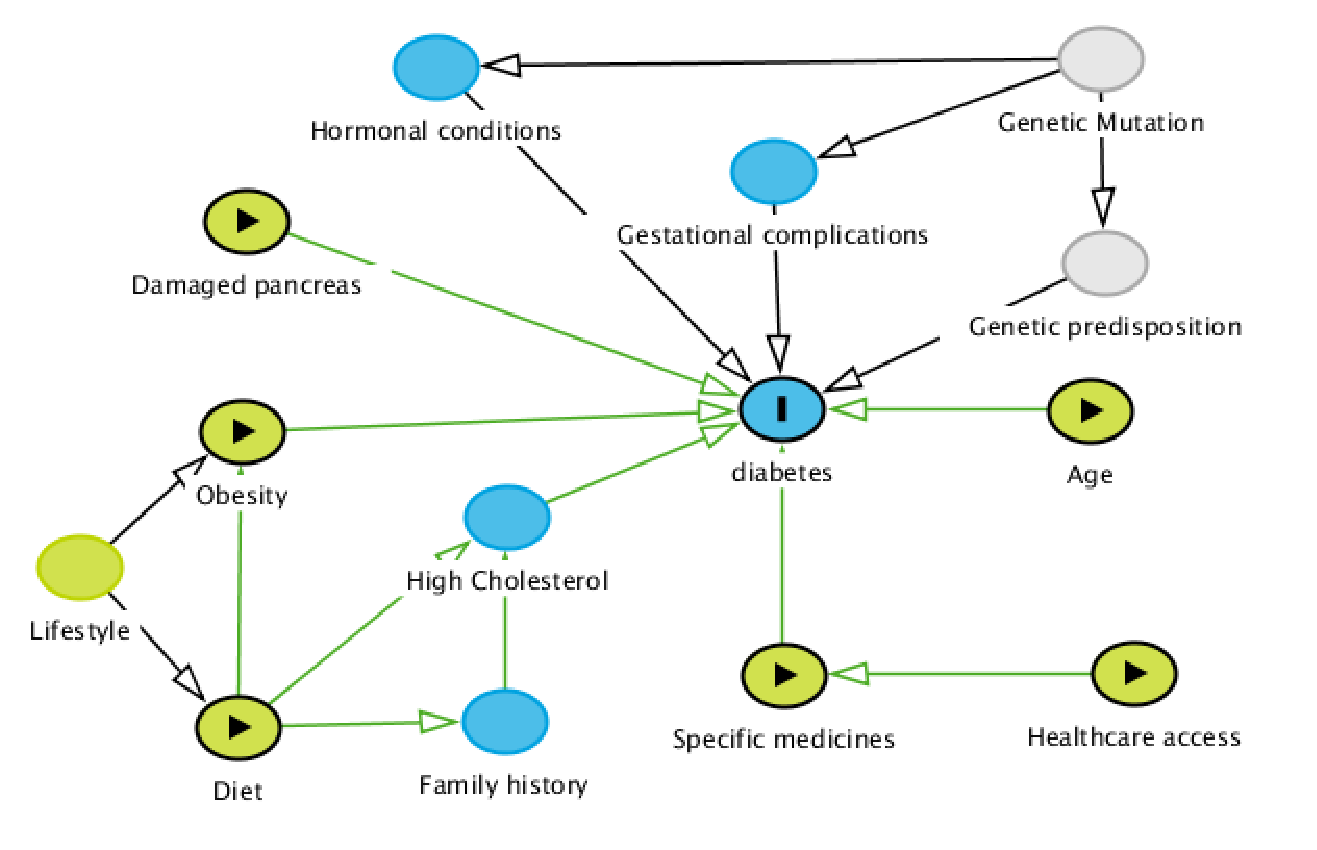
\includegraphics[width=\textwidth]{diabetes-causalmodel.eps}
	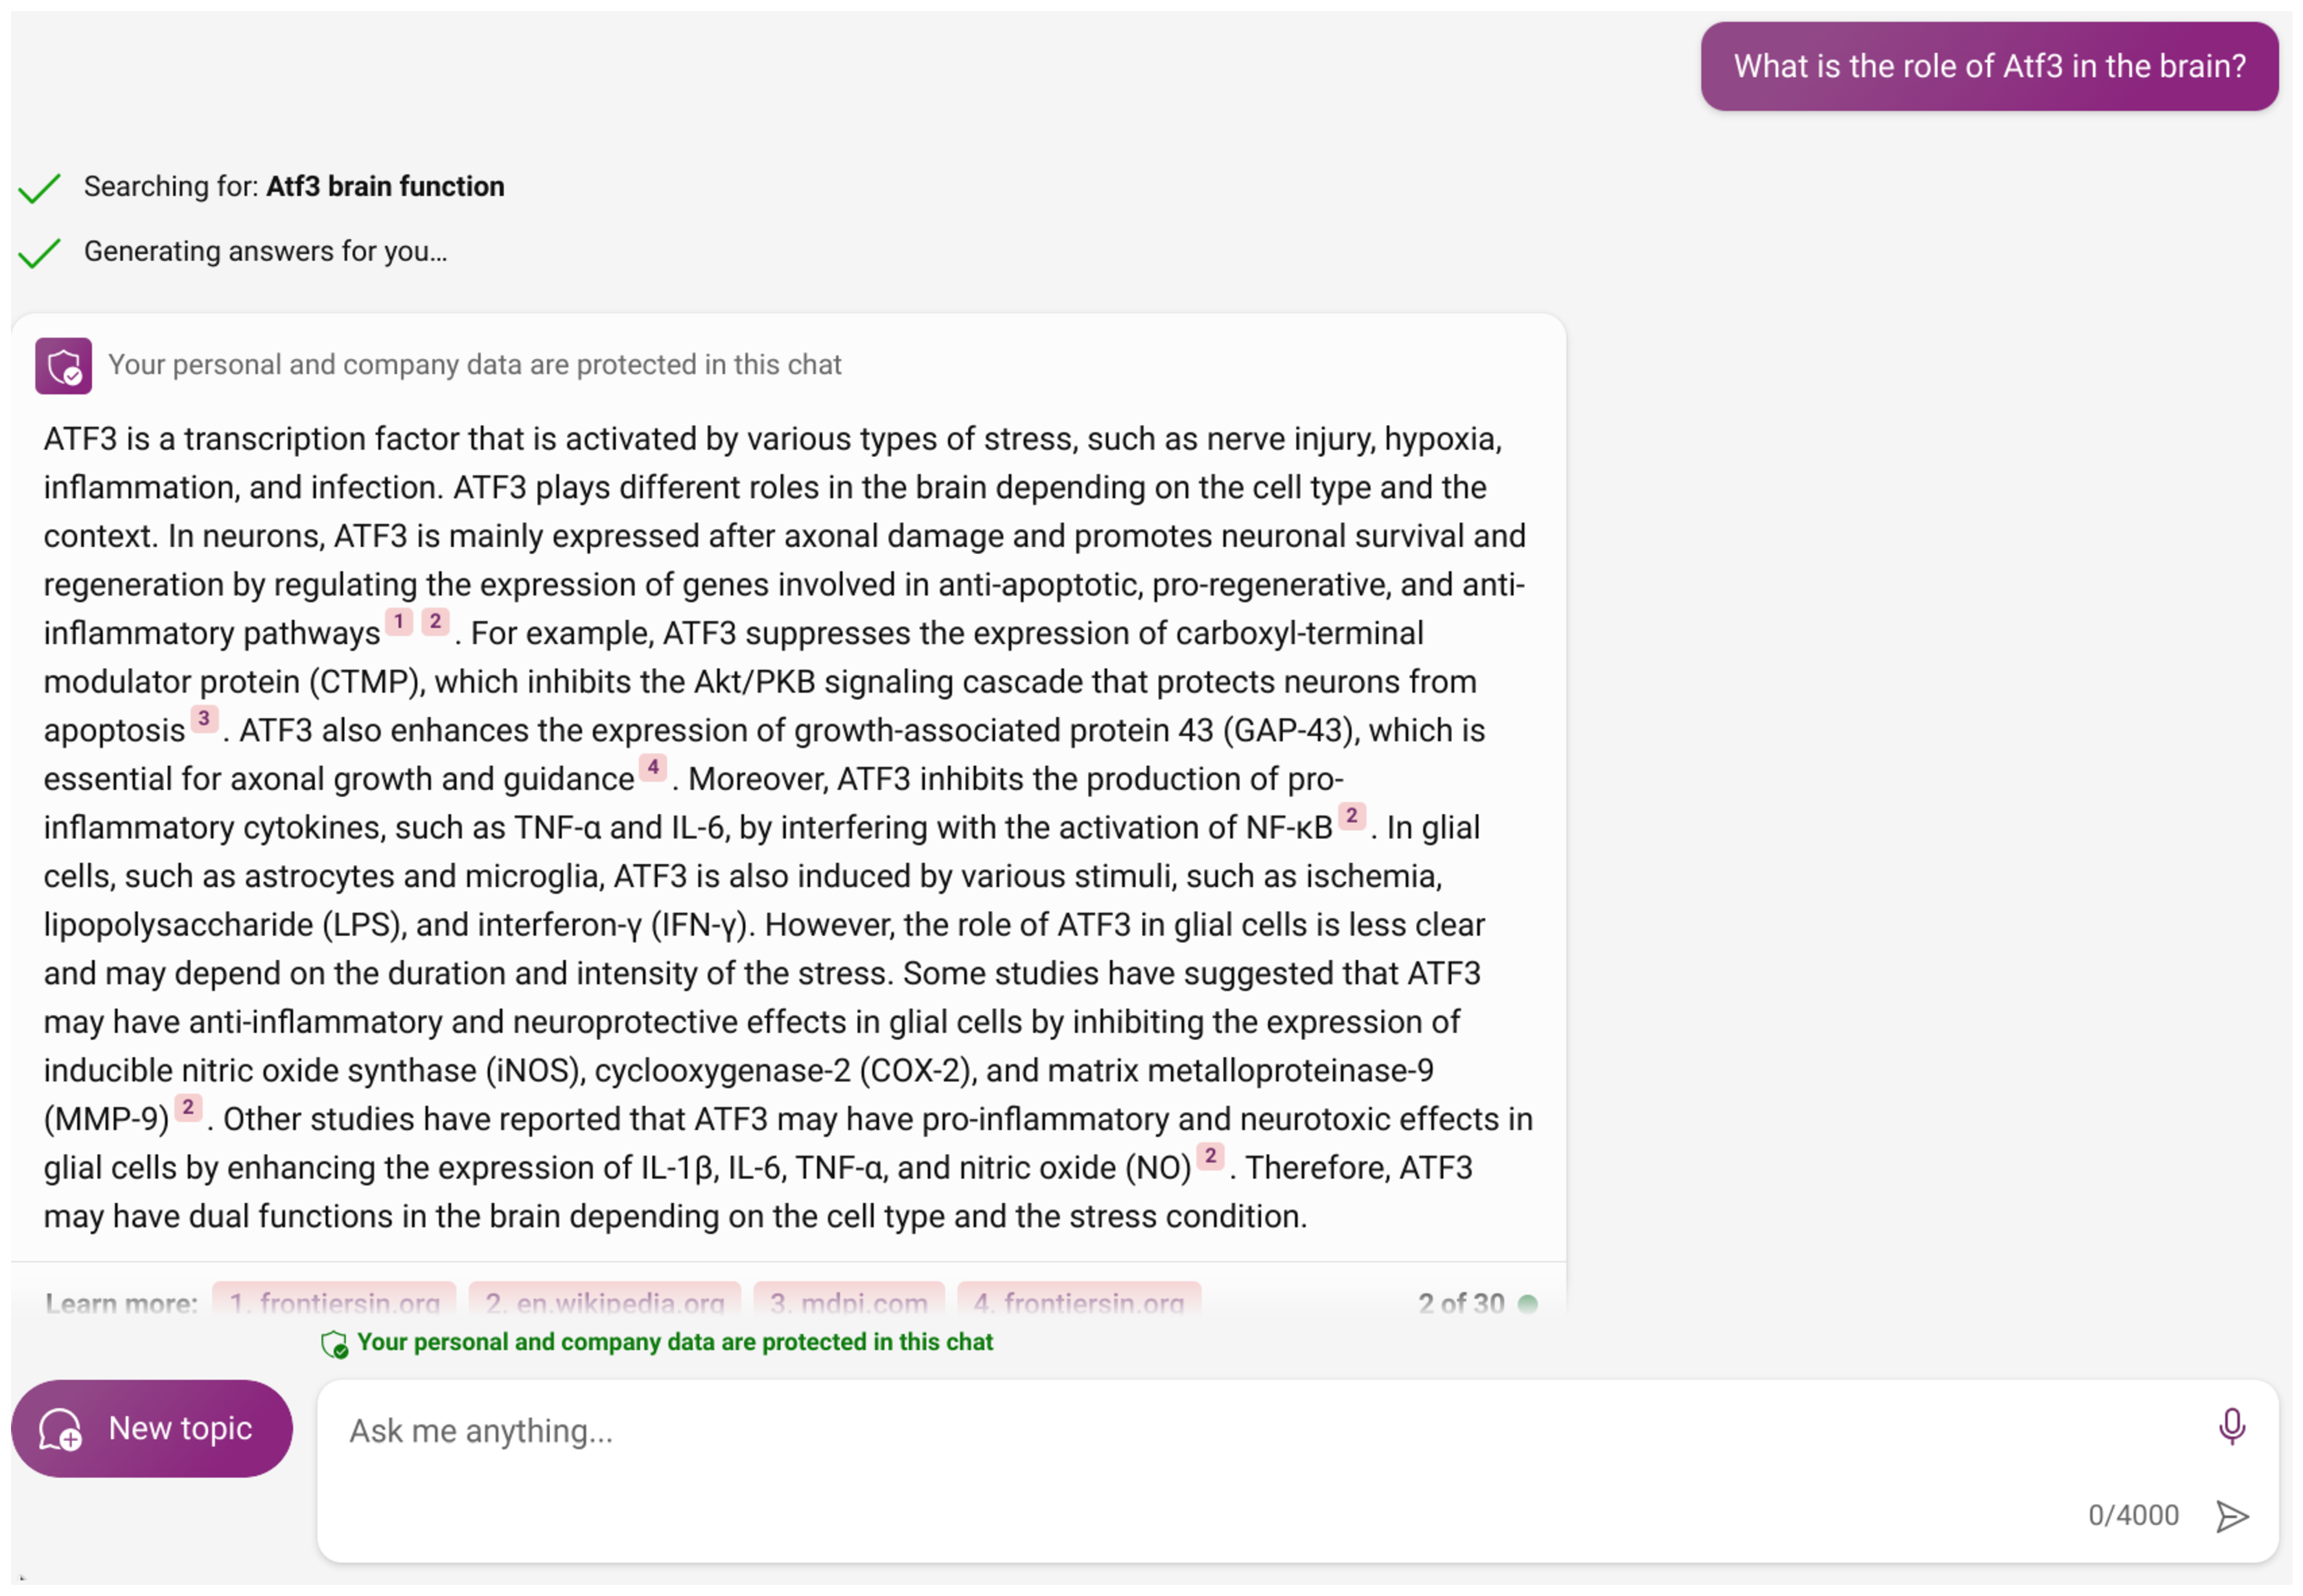
\includegraphics[width=.5\textwidth]{bingchat_atf3.eps}
	\caption{ \textbf{Bing Chat Query and Answer Example}
    The same question was asked BingChat and the existing demo of GNQA: `What is the role of Atf3 in the brain?'. 
            }
        \label{fig:atf3-chatcomparison}
\end{figure}


Bing's chat interface combines with it search, making it similar to what we have envisioned. 
Bing is using its search as an Oracle as when asked biological questions it returns answers from wikipedia.org and popular scientific publishing houses, as can been seen in figure~\ref{fig:atf3-chatcomparison}.
We want the GeneNetwork Question and Answer system to work similarly where search and summarization are handled and combined in a response.
The current version of our question answering system returns multiple references with each response, and will later return links to papers in PubMed and other refernce sites, along with links to datasets when sensible.

%\newpage
%\captionsetup{font={scriptsize,sc,up,singlespacing}}
\begin{figure}[h] % Figure at bottom of the page ([b] argument, could be "t" for top or "h" for here)
	\centering
	%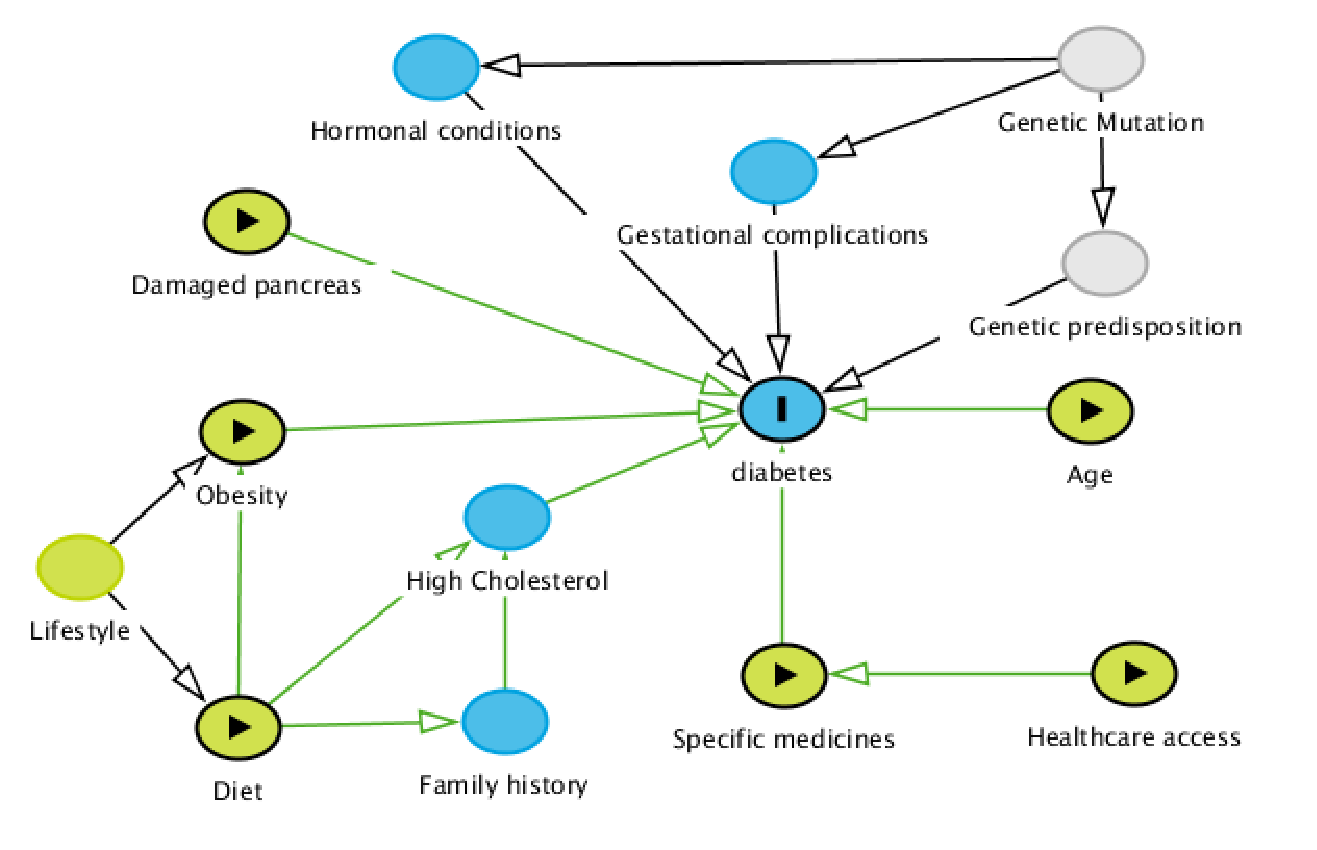
\includegraphics[width=\textwidth]{diabetes-causalmodel.eps}
	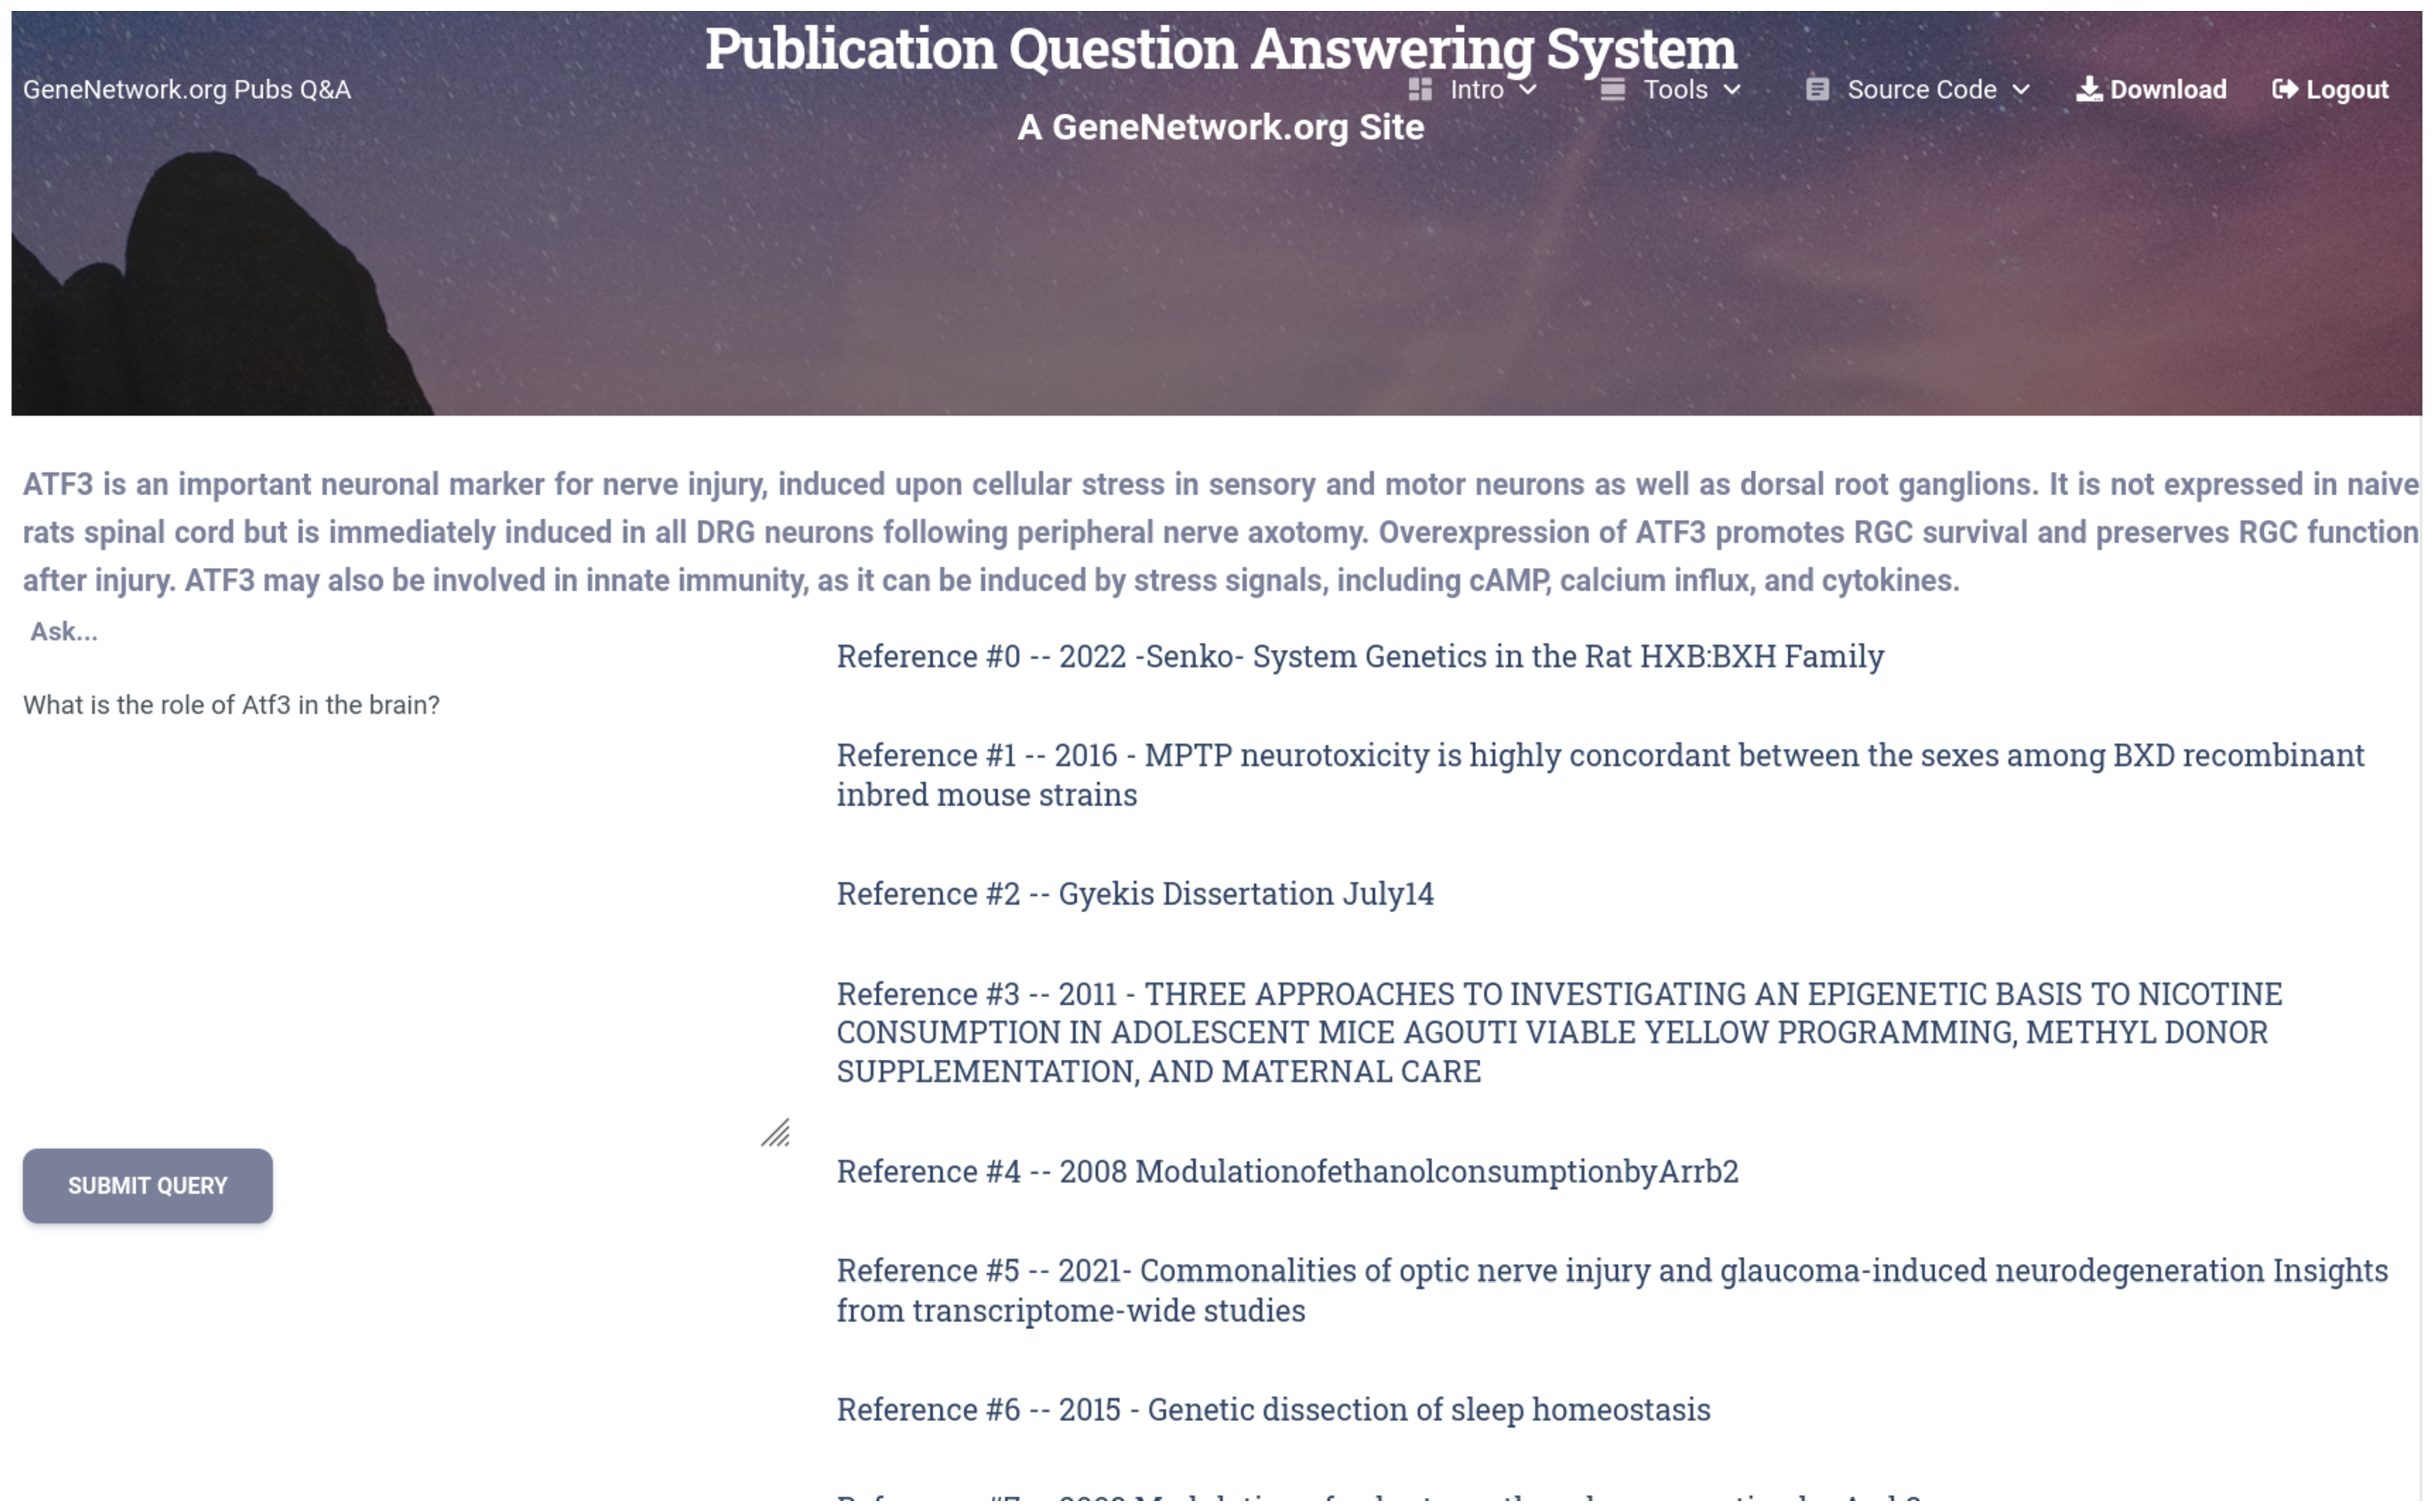
\includegraphics[width=.5\textwidth]{gnqa_atf.eps}
	\caption{ \textbf{GeneNetwork.org Query and Answer Example}
    The same question was asked BingChat and the existing demo of GNQA: `What is the role of Atf3 in the brain?'. 
            }
        \label{fig:gnqa_atf}
\end{figure}


Looking at figure~\ref{fig:gnqa_atf} one can see that references are returned with summaries for immediate further reading.
The systems development will later include links to other sites with scientific works and datasets on which studies and experiments have been conducted, from the publications of interest that have used the \GN\ database.
Our system is meant to be a support tool for researchers while being a tool that can help a novice or citizen scientist learn more about \GN\ research.

\section{GNQA: A Development Roadmap}
There are 3 major development phases for this system:
\begin{enumerate}
    \item Design and development of a fully-functioning question answering system using OpenAI's APIs, along with software oracles
    \item Build our own LLM using OSS software and techniques; therefore, replacing OpenAI's system
    \item Incorporate other OSS LLM projects as necessary
\end{enumerate}

Each of these development phases is a significant research and development undertaking that will be published and help push forward research and research access in the age of high-performing large language models.
In addition for each phase of development we will define and adhere to specific performance and satisfaction evaluations; including ease of use, usability and utility.


As far as computational intelligence researchers are concerned, the techniques pursued and implemented will be a part of the road-map to artificial general intelligence.

%\subsection{What lessons were learned from IBMs 2010 super AI system, Watson?}


\subsection{Optimizing an LLM for research that uses the GeneNetwork Genomics database}

As recognized by other researchers, specifically \cite{Tan:2017}, data acquisition is one of the most important aspects of any expert system. 
Before building every component of the expert system we will test and optimize the major components one at a time.
By utilizing existing tools and LLM's we will load hundreds of documents with an overall specified area on which we want the system to be an expert.
This work focuses on the Web QTL or GeneNetwork.org genomic database containing many terabytes of rat and mouse genomic information, as referenced by many \cite{Chesler:2004,Alberts:2010} \cite{Alberts:2010} \cite{Mulligan:2017} \cite{Watson:2020}.

\subsubsection{How it's going}
At the moment oracles have not been added to the system, we have submitted 950 publications to tune an LLM.
All of the articles are either about GeneNetwork.org or use its data.
The system uses the following models: [ask Adrian to provide the information].

A biologist has been able to test the system and asked it a range of questions.
Their aim was to get a comprehensive understanding of what the types of questions the system ``should'' be able to answer.
The investigators' questions and comments come from their frame of reference, specifically whether or not the system is answering questions correctly and whether the response, if not a direct answer, will be able to lead one to the truth.
%, then compared its responses to asking \openai's GPT3.5 model directly.
Summarization and inference abilities were tested through the investigators questions.
A full transcription of the questions and the investigators comments can be found in the appendix.% add a reference
This system needs to show more specific knowledge about genomics research with respect to rats and mice, as the same is the focus of the data on GeneNetwork.org.

%Shelby Solomon Darnell will have to run drills using workman.
\subsection{LLM development for full system reproducibility}
The current \project\ interfaces with an application programming interface (API) provided by \openai\ by way of FahamuAI, a Kenyan company specializing in artificial intelligence system development.
In order to have reproducible code, down the byte and bit levels, we use \guix, an open source package management system that also can use containers to run software \cite{Vallet:2022_guix}.
\subsection{Adding tools as we go, OSS LLMs projects}
% Including more OSS LLM projectssoftware oracles}
Since \openai\ proved the ability and performance of its ChatGPT platform, the proliferation of tools being developed that utilize generative AI has grown exponentially.
A site `futurepedia.io' keeps track of new LLM tools on a daily basis.
As of the 8th of September 2023, there are 5014 tools listed on the site.
In addition to the tools advertised on the site, there are many other projects that are not `full-blown' or `commercial level', while being very useful.

\section{ Acknowledgments}
Many thanks to the Kenyan startup `Fahamu AI' that helped us demo the first version of the GeneNetwork Question Answering system.

%\bigskip
%\noindent Thank you for reading these instructions carefully. We look forward to receiving your electronic files!

\begin{small}
\bibliographystyle{aaai}
\bibliography{refs/scholar, refs/blog, refs/causal, refs/gn}
\end{small}

%\clearpage
\newpage
\appendix
\appendixpage
\section{GeneNetwork.org Q\&A System}
%\appendixname{GeneNetwork.org Q\&A Testing}
%\section{GeneNetwork.org Q\&A Testing}

\begin{tabular}{|l|c|c|} 
    \hline
    \textbf{Data type} & & \textbf{Data representation} \\
    \hline\hline
    Query text & $-->$ & \cyan{Light blue/Cyan}  \\
    System Reply text & $-->$ & \violet{Responses are violet}  \\
    Biologists comments & $-->$ & \brown{\textit{Brown italics}}\\
    \hline
\end{tabular}


%\fbox{\parbox{\textwidth}{
%\paragraph*{}

\cyan{What is the most recent paper published using the BXD population?} \\

\violet{The most recent paper published using the BXD population is from 2018.} \\
\violet{The most recent paper published using the BXD population is from 2019.} \\

\brown{\textit{I am assuming the two different responses (some days apart) are because the database of papers is being actively expanded.
I can’t actually verify the LLMs statement as the citation information is not exposed yet (just a hash). 
The top hit quotes from David’s ‘expanded BXD family’ paper from 2019, so it seems OK. 
Not sure why there is more than one hit for this query though (is the LLM actually collecting dates and finding the max? Or is it just making up text?)}}

\cyan{How many strains are available for the BXD population?}

\violet{There are a totoal of 123 BXD strains available.}

\brown{\textit{I have received some different values, but all under the 150 quoted in David's 2019 paper (which we know from above is in the reading list).}}

\cyan{How are C57BL/6 and DBA/2 different?}

\violet{C57BL/6 and DBA/2 differ in their ability to respond to xenobiotics.}

\brown{\textit{I saw some different responses, all quoed from single references - not a summary as I would have liked to see.}}

%--------------------------------------------------------------

\cyan{Is C57BL/6 smarter than DBA/2?}

\violet{There is no mention of intelligence in the text.}

\brown{\textit{OK - fair enough. ChatGPT gives a lyrical response about the multifaceted nature of intelligence. Not sure which is more honest :) This was a stupid question anyway just to test the breath of the summarising abilitis.}}

%--------------------------------------------------------------

\cyan{Which mouse strain has the biggest brain?}

\violet{The C57BL/6J (C57) mouse strain has the biggest brain.}

\brown{\textit{This is broadly true I think, in the realm of standard strains.}}
%}}
%--------------------------------------------------------------
%\fbox{\parbox{\textwidth}{
%\paragraph*{}

\cyan{What is the typical weight of a mouse liver?}

\violet{The average liver weight in a normal mice is 10 mg per g wet weight.}

\violet{The average weight of a mouse liver is 3.5 grams.}

\brown{\textit{Two very different answers on different days. Both wrong. I thought this would be one that an LLM could deal with.}}

%--------------------------------------------------------------

\cyan{What behavioural QTLs have been found in mice?}

\violet{Two QTLs located on chromosomes 1 and 5 modulate different aspects of the
performance of mice of the B x D Ty RI strain series in the Morris navigation task.}

\brown{\textit{Sounds like it has been ripped verbatim from a single paper.
Edit: Yes, this is from reference \#3.
“Two QTLs located on chromosomes 1 and 5 modulate different aspects of the performance
of mice of the BXD Ty RI strain series in the Morris navigation task. Behav Genet. 2002;
32:6978. [PubMed: 11958544] Mozhui RT, Ciobanu DC, Schikorski T, Wang XS, Lu L,
Williams RW. Dissection of a QTL hotspot on mouse distal chromosome 1 that modulates
neurobehavioral phenotypes and gene expression. PLoS Genetics. 2008; 4:e1000260.
[PubMed: 19008955] Mulligan MK, Wang X, Adler AL, Mozhui K, Lu L, Williams RW.
Complex control of GABA(A) receptor subunit mRNA expression: variation, covariation, and
genetic regulation. PLoS One. 2012; 7(4):e34586.”
Here, it looks like a part of the References section has been used in the text mining. That is a
problem if the aim mis to link statements to correct citations. I don’t know what the source
reference is (still just a hash) but it is very likely NOT the source of the response text.}}
%}}
%--------------------------------------------------------------

%\fbox{\parbox{\textwidth}{
%\paragraph*{}
\cyan{What are these QTLs?}

\violet{These QTLs are stretches of DNA that are closely linked to genes that underlie a phenotype of interest.}

\brown{\textit{I was hoping for more information about the previous query. I got basically the same response when asking the same question in a different session though, so there is no evidence of contextual memory. I didn’t pursue this further.}}

%--------------------------------------------------------------

\cyan{What does QTL mean?}

\violet{[Quantitative trait locus (QTL) is a gene or group of linked genes that influence a
quantitative trait.}

\brown{\textit{OK, but weak answer given that this is exactly the sort of situation wher an LLM
should shine.
Would it perhaps make sense to give the LLM the FAQ data as part of its training?}}

%--------------------------------------------------------------

\cyan{What is the role of Atf3 in the brain?}

\violet{Atf3 is a transcriptional activator that binds to the cAMP-responsive element (Cre). Interaction with Jun redirects Jun to bind to Cres preferentially over the 12-Otetradecanoylphorbol-13-acetate response elements (Tres) as part of an Atf2-c-Jun complex (487 aa). However, human study did not show strong support for the
association between ATF2 and alcoholism. Alcoholism is particularly influenced by the environment.}

\brown{\textit{The response seemed to come only from individual studies rather than being a summary of the field. That may be due to the small post-training dataset at this stage. Is there a 'relevance score' for the papers returned? Several references (and part of the response) were based on Atf2. This is a different gene. Does the system perform grounding to biomedical ontologies? Or is it just looking at text similarity (like Levenshtein distance)?}}

%--------------------------------------------------------------

\cyan{What is the NCBI GeneID four mouse ATf3?}

\violet{The NCBI GeneID for mouse Atf3 is ENSMUSG00000027109.}

\brown{\textit{Close, but no cigar. We got a gene ID for a mouse transcription factor, but that's all.
ENSMUSG00000027109 is mouse Sp3.}}

%}}
%--------------------------------------------------------------
%\fbox{\parbox{\textwidth}{
%\paragraph*{}

\cyan{What is the ENSEMBL GeneID for mouse Atf3?}

\violet{The ENSEMBL GeneID for mouse Atf3 is ENSMUSG00000064371.}

\brown{\textit{Nope, this is mitochondrial tRNA threonine.
I wasn’t expecting much from this query as we know this is NOT what LLMs do well. Maybe there could be re-training on the NCBI/Uniprot descriptions and even GeneRIF. I still think there should be a way to directly link entities to databases though.}}

%--------------------------------------------------------------

\cyan{What is the ENSEMBL identifier for Atf3 in mice?}

\violet{The ENSEMBL identifier for Atf3 in mice is ENSMUSG00000027109.}

\brown{\textit{Rephrasing the question gives qualitatively different answers. The citations are all kind of sane though. They actually do get close to Atf3 and the IDs appear to be drawn from these sources. Some explicit grounding would nail this down I think.}}
%}}
%--------------------------------------------------------------

%\fbox{\parbox{\textwidth}{
%\paragraph*{}
\cyan{Where can I find the ENSEMBL identifier for a gene such as Atf3?}

\violet{The ENSEMBL identifier for a gene can be found in the Affymetrix (June 2005 Annotation) and Ensembl AffyProbe (v33) databases.}

\brown{\textit{Hmm - yeeees, you COULD find the identifier there. But that is not where we should be looking. As a comparison, I ran the same query through ChatGPT (3.5):}} \red{\textit{As of my last knowledge update in September 2021, the gene Atf3 is indeed present
in the ENSEMBL database, but please note that information might have changed since then. To find the ENSEMBL identifier for the Atf3 gene, you can follow these steps:
1. Visit the ENSEMBL website: Go to the ENSEMBL website at
https://www.ensembl.org/.
2. Search for the gene: In the search bar at the top of the page, enter "Atf3" and press Enter or click the magnifying glass icon.
3. Select the gene: From the search results, you should find "Atf3" listed. Click on the gene name to access its detailed information page.
4. Find the ENSEMBL identifier: On the gene's page, you should be able to
find the ENSEMBL identifier (also known as the ENSEMBL Gene ID or ENSGID) listed in the gene's summary information or on the "Gene" section of the page. Please note that the specific layout of the ENSEMBL website and the location of information might have changed since my last update. If you're having trouble locating the ENSEMBL identifier or if you want the most up-to-date information, I recommend visiting the ENSEMBL website directly and using their search and navigation tools to find the gene Atf3 and its corresponding ENSEMBL identifier.}}
%}}
%--------------------------------------------------------------
%\fbox{\parbox{\textwidth}{
%\paragraph*{}
\cyan{Where do I look for genes that regulate hippocampal neural stem cell proliferation?}

\violet{In the QTL region.}

\brown{\textit{Obviously :D. I was expecting something more along the lines of the ChatGPT response, that pointed me (in a generic way) to a bunch of sensible resources.}}

%--------------------------------------------------------------

\cyan{}

\violet{}

\brown{\textit{}}
%}}


\end{document}